\documentclass[10pt]{beamer}
\usepackage[T2A]{fontenc}                
\usepackage[utf8]{inputenc}  
\usepackage[english, russian]{babel}
\usepackage{indentfirst}
\usepackage{graphicx}
 
\usetheme{Szeged}
\usecolortheme{wolverine}

\title{Пакеты Прикладных Программ \\ Отчет по второму этапу}
\author{Юмашев Артем и Чабан Олег}
\institute{ВМК МГУ}
\date{2017}
 
\begin{document}
 
\frame{\titlepage}
 
\begin{frame}
\frametitle{Постановка задачи}
После оглушительного успеха в освобождении Астапора, Миэрина и Юнкая от власти работорговцев Дейенерис Бурерожденная открыла себе доступ к Летнему морю, а следовательно -- путь в Вестерос.\\
Для ведения войны с Семью Королевствами нужно оружие, а для оружия нужна сталь. Нет никаких сомнений в кузнечном искусстве Безупречных, однако поставщики стали не столь надежны.\\
Два основных поставщика стали -- это {Westeros Inc.} и {Harpy \& Co}. На протяжении нескольких месяцев мы закупаем сталь у обеих компаний, и каждая из них предлагает ощутимую скидку при заключении эксклюзивного договора на поставку.\\
\end{frame}

\begin{frame}
\frametitle{Постановка задачи}
Советник королевы Тирион Ланнистер знает о твоем умении принимать взвешенные рациональные решения и просит помощи в объективном решении вопроса о том, с какой из компаний следует заключить эксклюзивный договор на поставку стали.\\
У Тириона есть записи о производстве мечей каждым из кузнецов-безупречных, а также данные о количестве сломанных мечей в каждый из месяцев ведения боевых действий.\\
\end{frame}
 
\begin{frame}
\frametitle{Цель работы}
Необходимо провести разведывательный анализ данных с целью ответа на вопрос: "С каким из поставщиков стали следует заключить договор?". Наш горизонт планирования составляет 11 месяцев. Вместе с данными за прошедшие 7 месяцев из CSV-файла, планируемое время ведения боевых действий составляет полтора года.
\end{frame}

\begin{frame}
\frametitle{Алгоритм работы}
\begin{enumerate}
\item Считываем данные из CSV-файла.
\item Задаем переменные и их значения.
\item Заполняем векторы harpy и westeros.
\item Строим диаграмму размаха.
\end{enumerate}
\end{frame}

\begin{frame}
\frametitle{Обоснование выбора метода}
Будем исследовать эффективность производства каждой компании при помощи диаграммы размаха или "ящиков с усами". Так называют графики, использующиеся в описательной статистике, компактно изображающий одномерное распределение вероятностей. Такой вид диаграммы в удобной форме показывает медиану (или, если нужно, среднее), нижний и верхний квартили, минимальное и максимальное значение выборки и выбросы. Несколько таких ящиков можно нарисовать бок о бок, чтобы визуально сравнивать одно распределение с другим; их можно располагать как горизонтально, так и вертикально. Расстояния между различными частями ящика позволяют определить степень разброса (дисперсии) и асимметрии данных и выявить выбросы.
\end{frame}

\begin{frame}
\frametitle{Ход работы}
На оси абсцисс в нашей задаче укажем названия компаний (harpy.co и westeros.inc), на оси ординат --- значения векторов количества целых мечей, заполненных следующим образом:\\~\\
В качестве элемента будем брать разность количества произведенных мечей от конкретной партии и количества сломанных мечей. Эти значения суммируются по всем работающим в конкретной компании кузнецам.
\end{frame}

\begin{frame}
\frametitle{Ход работы}
~\\
Построим диаграммы размаха.
\begin{figure}
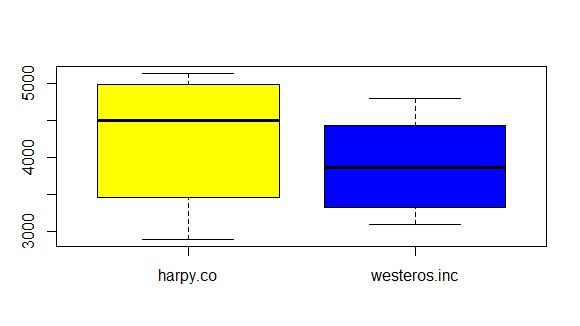
\includegraphics[width=80mm]{boxes.jpg}
\caption{Ящики с усами}
\label{boxes}
\end{figure}
\end{frame}

\begin{frame}
\frametitle{Анализ полученных результатов}
Изучив график можно сказать, что:\\
Качество мечей у Harpy \& Co выше, нежели качество мечей Westeros Inc., так как медиана первого ящика находится выше, нежели медиана второго ящика.\\
В то же время, качество партий Westeros Inc. выше, чем качество партий Harpy \& Co, так как разброс минимального и максимального количества целых мечей у первой компании меньше, нежели у второй.
\end{frame}

\begin{frame}
\frametitle{Вывод}
Изучив все данные, и зная, что наш горизонт планирования составляет 11 месяцев, можно сказать, что будем делать вывод, основываясь на значении медианы. Поэтому мы можем посоветовать Тириону Ланистеру довериться компании Harpy \& Co и заключить с ними контракт, не боясь, что он потом вызовет нас на суд поединком.
\begin{figure}

\includegraphics[width=40mm]{tirion.jpg}
\end{figure}
\end{frame}

\begin{frame}{Задание выполняли}
	\begin{itemize}
		{\small
		\item Юмашев Артем. Написание программы, написание отчета в Rnotebook.
		\item Чабан Олег. Написание презентации.
		}
	\end{itemize}	

\end{frame}

\end{document}